\chapter{Identieke deeltjes}\label{ch:b3:identical-particles}

Elk elektron in het heelal is strikt en volmaakt identiek aan elk ander
--- niet gelijkend zoals twee munten uit één munthuis, maar in beginsel
niet te onderscheiden: geen etiket, geen kras, geen geschiedenis kan er
één merken. De kwantummechanica neemt dat serieus, en de gevolgen
besturen de wereld. Twee \omterm{def:b3:identical-particles:exchange}{identieke deeltjes} verwisselen mag niets
waarneembaars veranderen, en dat laat de veeldeeltjesgolffunctie maar twee
mogelijkheden: hetzelfde blijven (\emph{bosonen}) of van teken wisselen
(\emph{fermionen}). Uit het minteken alleen volgen het
\omterm{cor:b3:identical-particles:pauli}{uitsluitingsbeginsel van Pauli}, de schilstructuur en het hele \omterm{prop:b3:identical-particles:periodic}{periodiek
systeem}, de stevigheid van de materie onder onze voeten, en de druk die
dode sterren overeind houdt; uit het plusteken volgen de
gezelligheidsdrang van fotonen --- vandaar de laser --- en, drie
hoofdstukken verderop, de bose-einsteincondensatie. Zelden heeft in de
natuurkunde één teken zoveel gedragen.

\section{Het symmetriseringspostulaat}

\begin{definition}[Verwisseling]\label{def:b3:identical-particles:exchange}
\index{identieke deeltjes}\index{verwisselingsoperator}
Voor twee identieke deeltjes met een toestandsruimte opgespannen door
producten $\ket{a}\otimes\ket{b}$ (deeltje 1 in $\ket a$, deeltje 2 in
$\ket b$ --- posities, spins en al) verwisselt de
\emph{verwisselingsoperator} $\hat P_{12}$ de rollen: $\hat P_{12}\ket a\otimes\ket b =
\ket b\otimes\ket a$. Hij is hermitisch, kwadrateert tot
de identiteit en commuteert met elke \omterm{def:b3:hamiltonian-mechanics:hamiltonian}{hamiltoniaan} die de deeltjes
identiek behandelt: zijn \omterm{def:b3:quantum-formalism:observable}{eigenwaarden} $\pm1$ zijn behouden etiketten van
de wereld.
\end{definition}

\begin{theorem}[Bosonen en fermionen]\label{thm:b3:identical-particles:postulate}
\index{boson}\index{fermion}\index{spin-statistiekstelling}
Toestanden van \omterm{def:b3:identical-particles:exchange}{identieke deeltjes} mogen niet alleen eigentoestanden van
elke verwisseling zijn, zij \emph{moeten} het zijn: volledig
\emph{symmetrisch} voor de ene klasse deeltjes --- de \emph{bosonen} ---
en volledig \emph{antisymmetrisch} (een tekenwissel bij elke
verwisseling) voor de andere --- de \emph{fermionen}. Tot welke klasse een
soort behoort ligt vast door haar spin (de
\emph{spin-statistiekstelling}, alleen in de relativistische
kwantumveldentheorie bewezen en hier aangenomen):
\[
\text{gehele spin} \Rightarrow \text{boson} , \qquad
\text{halftallige spin} \Rightarrow \text{fermion} .
\]
Fotonen, pionen en $^4$He-atomen zijn bosonen; elektronen, protonen,
neutronen en $^3$He zijn fermionen.
Een samengesteld deeltje gedraagt zich als de som van zijn delen: een
even aantal samengebonden fermionen is een boson ($^4$He: 2p + 2n + 2e),
een oneven aantal een fermion ($^3$He) --- met gevolgen die zo zichtbaar
zijn als twee verschillende vloeibare heliums.
\end{theorem}
\admitted

\begin{corollary}[Het uitsluitingsbeginsel van Pauli]\label{cor:b3:identical-particles:pauli}
\index{uitsluitingsbeginsel van Pauli}
Twee fermionen kunnen nooit dezelfde eendeeltjestoestand bezetten:
$\ket a = \ket b$ in de antisymmetrische combinatie
$(\ket a\otimes\ket b - \ket b\otimes\ket a)/\sqrt2$ invullen geeft de
nulvector --- zo'n toestand bestaat niet. Voor elektronen (spin
$\tfrac12$) laat elke orbitaal er hoogstens twee toe, met tegengestelde
spinprojectie.
\end{corollary}

\begin{example}[Anders tellen]\label{ex:b3:identical-particles:counting}
Twee deeltjes over twee toestanden $a, b$: klassiek (onderscheidbaar)
tellen geeft vier configuraties; bosonen hebben er drie ($aa$, $bb$ en
\emph{één} gemengde toestand); fermionen precies één (de gemengde,
antisymmetrische). De statistische fysica zal deze tellingen ongewijzigd
overnemen (\cref{ch:b3:quantum-statistics}); hier lossen zij al een
negentiende-eeuwse gêne op --- de entropie van het ``mengen'' van twee
monsters van hetzelfde gas
(\cref{exo:b3:identical-particles:10}).
\end{example}

\section{Het periodiek systeem}

\begin{proposition}[Schillen, en waarom er scheikunde bestaat]\label{prop:b3:identical-particles:periodic}
\index{periodiek systeem}\index{opbouwbeginsel}
Vul de waterstofachtige orbitalen $(n, l, m, m_s)$ met telkens één
elektron, de laagste energieën eerst, in de niveauvolgorde die door
doordringing en afscherming wordt bepaald ($1s$, $2s$, $2p$, $3s$, $3p$,
$4s$, $3d$, \dots --- \cref{exo:b3:hydrogen-atom:8}). Het beginsel van
Pauli laat het vullen \emph{verzadigen}: $2$ elektronen sluiten de eerste
schil, $8$ de tweede en de derde rij, en de tabel van de elementen krijgt
haar perioden. De scheikunde is de natuurkunde van welke elektronen het
uitsluitingsbeginsel ook maar het buitenst heeft achtergelaten: volle
schillen (edelgassen) zijn traag; één elektron boven een volle schil
(alkalimetalen) of één gat tekort (halogenen) is op tegengestelde wijze
reactief. Zonder het minteken zou elk elektron in $1s$ wegzakken, zou elk
atoom een geschrompelde heliumachtige bol zijn, en zouden er geen
bindingen, geen moleculen en geen scheikundigen zijn om er spijt van te
hebben.
\end{proposition}
\admitted

\begin{omfigure}
\begin{tikzpicture}[font=\small, >=Stealth]
  % 1s
  \draw[thick] (0,0) rectangle (1.0,0.7);
  \node[anchor=north] at (0.5,-0.08) {$1s$};
  \node at (0.5,0.35) {$\uparrow\downarrow$};
  % 2s
  \draw[thick] (1.9,0) rectangle (2.9,0.7);
  \node[anchor=north] at (2.4,-0.08) {$2s$};
  \node at (2.4,0.35) {$\uparrow\downarrow$};
  % 2p: three boxes
  \foreach \i in {0,1,2} \draw[thick] ({3.5+\i*1.05},0) rectangle ({4.5+\i*1.05},0.7);
  \node[anchor=north] at (5.05,-0.08) {$2p$ (drie orbitalen)};
  \node at (4.0,0.35) {$\uparrow\downarrow$};
  \node at (5.05,0.35) {$\uparrow$};
  \node at (6.1,0.35) {$\uparrow$};
  \node[anchor=west, align=left, font=\footnotesize] at (7.4,0.35)
    {zuurstof ($Z = 8$): $1s^2\,2s^2\,2p^4$\\
     evenwijdige spins spreiden zich eerst\\ (regel van Hund)};
  \draw[decorate, decoration={brace, mirror, amplitude=4pt}] (0,-0.65) -- (2.9,-0.65);
  \node[font=\footnotesize] at (1.45,-1.05) {gesloten bij He en Be};
  \draw[decorate, decoration={brace, mirror, amplitude=4pt}] (3.5,-0.65) -- (6.55,-0.65);
  \node[font=\footnotesize] at (5.05,-1.05) {gesloten bij Ne: scheikunde voorbij};
\end{tikzpicture}

{\small De orbitalen twee aan twee vullen: het uitsluitingsbeginsel bouwt
de perioden van de tabel. De vier $2p$-elektronen van zuurstof
illustreren de regel van Hund --- spins lijnen uit en spreiden zich over
de orbitalen voordat zij zich paren, een zuiver verwisselingseffect
(\cref{prop:b3:identical-particles:exchange-force}).}
\end{omfigure}

\section{De verwisselingswisselwerking}

\begin{proposition}[Symmetrie van de ruimtelijke paartoestand]\label{prop:b3:identical-particles:exchange-force}
\index{verwisselingswisselwerking}
Voor twee elektronen moet de totale toestand (ruimte $\times$ spin)
antisymmetrisch zijn: een \emph{singlet} (antisymmetrische spin,
\cref{exo:b3:spin-two-level:11}) dwingt een \emph{symmetrische}
ruimtelijke golffunctie af, een \emph{triplet} een antisymmetrische. De
twee verschillen natuurkundig: in de antisymmetrische ruimtelijke
toestand kunnen de elektronen nooit samenvallen ($\psi(\vect r, \vect r) = 0$) en houden zij afstand, terwijl de symmetrische toestand ze laat
samendringen. Omdat nabijheid coulombenergie kost, krijgt de
spinopstelling een energieverschil --- de \emph{verwisselingsenergie} ---
van elektrostatische omvang (elektronvolts!), hoewel er geen magnetische
kracht van die sterkte bestaat: spins lijnen uit of tegen elkaar in door
meetkunde plus afstoting. Dit is de motor van de regel van Hund, van de
twee spectra van helium, van de covalente binding en --- door een kristal
heen opgeschaald --- van het ferromagnetisme zelf
(\cref{ch:b3:electromagnetism-in-matter}).
\end{proposition}

\begin{proof}[Gedeeltelijk bewijs]
De symmetrieboekhouding is
\cref{thm:b3:identical-particles:postulate} plus de spincombinaties; het
verdwijnen bij samenvallen is de antisymmetrie gelezen bij $\vect r_1 = \vect r_2$. Het energiegevolg is \omterm{thm:b3:perturbation-theory:corrections}{storingsrekening} van eerste orde in de
afstoting: de directe term is beide symmetrieën gemeen en de gekruiste
(``verwisselings'')integraal komt met tegengestelde tekens binnen
(\cref{exo:b3:identical-particles:6}).
\end{proof}

\begin{omfigure}
\begin{tikzpicture}
  \begin{axis}[omaxis, axis x line=bottom, axis y line=left,
    width=11.4cm, height=5.4cm, xmin=-3.4, xmax=3.4, ymin=0, ymax=1.28,
    xlabel={afstand $x_1 - x_2$ (willekeurige eenheden)},
    ylabel={paardichtheid},
    xlabel style={at={(axis description cs:0.5,-0.1)}, anchor=north},
    xtick=\empty, ytick=\empty, clip=false,
    legend style={font=\scriptsize, at={(0.98,0.76)}, anchor=north east,
      draw=none, fill=none}]
    \addplot[omThm, very thick, domain=-3.4:3.4, samples=120]
      {(1+exp(-x*x))*exp(-x*x/6)*0.62};
    \addlegendentry{symmetrisch (bosonen; singletelektronen)}
    \addplot[omDef, very thick, domain=-3.4:3.4, samples=120]
      {(1-exp(-x*x))*exp(-x*x/6)*0.9};
    \addlegendentry{antisymmetrisch (tripletelektronen)}
  \end{axis}
\end{tikzpicture}

{\small De kans om het paar op afstand $x_1 - x_2$ aan te treffen: de
symmetrische ruimtelijke toestand dringt bij contact samen, de
antisymmetrische draagt een ``verwisselingsgat'' --- exact nul bij
samenvallen. Voer die meetkunde aan de coulombafstoting en de
spinopstellingen krijgen energieverschillen van elektronvolts.}
\end{omfigure}

\begin{example}[De twee heliums in één atoom]\label{ex:b3:identical-particles:helium}
De aangeslagen toestanden $1s\,2s$ van helium komen in twee families die
elkaar nauwelijks kruisen: \emph{para}helium (singlet, symmetrische
ruimte) en \emph{ortho}helium (triplet, antisymmetrische ruimte), waarbij
het triplet $\approx\qty{0.8}{eV}$ \emph{lager} ligt --- zijn
verwisselingsgat bespaart coulombafstoting. De grondtoestand is
noodzakelijk para ($1s^2$ dwingt de symmetrische ruimtelijke toestand af);
en de laagste orthotoestand, zonder lager triplet om naar te vervallen en
met verboden spinomklappen, leeft uren --- een metastabiel atoom dat als
werkpaard in atoombundels dienstdoet. Negentiende-eeuwse spectroscopisten
catalogiseerden ``twee heliums''; de oplossing is één minteken.
\end{example}

\begin{example}[De covalente binding]\label{ex:b3:identical-particles:bond}
Breng twee waterstofatomen bij elkaar: de twee elektronen kunnen in de
symmetrische ruimtelijke combinatie van de twee atomaire orbitalen gaan
(spins in singlet) of in de antisymmetrische (triplet). De symmetrische
toestand hoopt lading \emph{tussen} de protonen op, waar zij beide
aantrekt: binding --- de covalente binding van H$_2$, \qty{4.5}{eV} diep.
De antisymmetrische toestand ontruimt het middenvlak: zuiver afstotend.
Elke regel van de organische scheikunde is boekhouding van elektronen met
gepaarde spins die symmetrisch worden gedeeld --- het uitsluitingsbeginsel,
achterstevoren gedraaid, is de lijm van de moleculen.
\end{example}

\section{Bosonen: hoe meer zielen, hoe meer vreugd}

\begin{proposition}[Bosonische versterking]\label{prop:b3:identical-particles:enhancement}
\index{gestimuleerde emissie!bosonische oorsprong}
Overgangen die een boson toevoegen aan een toestand die er al $n$ bevat
hebben amplitudes die met $\sqrt{n + 1}$ zijn versterkt --- tempo's met
$n + 1$ (de ladderalgebra van \cref{ch:b3:harmonic-oscillator}, want een
bosonische modus \emph{is} een oscillator). De ``$1$'' is de spontane
emissie; de ``$n$'' is de \emph{gestimuleerde} emissie, evenredig met de
menigte die er al is: de lawine achter elke laser (volume van jaar 2), nu
onthuld als zuivere verwisselingssymmetrie. Dezelfde statistiek,
toegepast op atomen die zijn gekoeld tot hun golfpakketten overlappen,
voorspelt een stormloop naar één enkele kwantumtoestand --- de
bose-einsteincondensatie, bewaard voor
\cref{ch:b3:quantum-statistics}.
\end{proposition}
\admitted

\begin{method}[Omgaan met identieke deeltjes]\label{met:b3:identical-particles:method}
(1) Bepaal de statistiek uit de spin (bij samengestelde deeltjes: tel de
fermionen op). (2) Splits voor twee elektronen ruimte $\times$ spin en
koppel de singlet aan een symmetrische ruimte en het triplet aan een
antisymmetrische. (3) Tel toestanden, nooit deeltjes-met-namen: maak een
lijst van bezettingen. (4) Energievragen met afstoting: de directe
integraal eenmaal, de verwisselingsintegraal met het teken van de
symmetrie. (5) Onthoud de twee spreuken --- fermionen: hoogstens één per
toestand, met een verwisselingsgat om elk; bosonen: tempo's opgevoerd door
de bezetting.
\end{method}

\begin{omfigure}
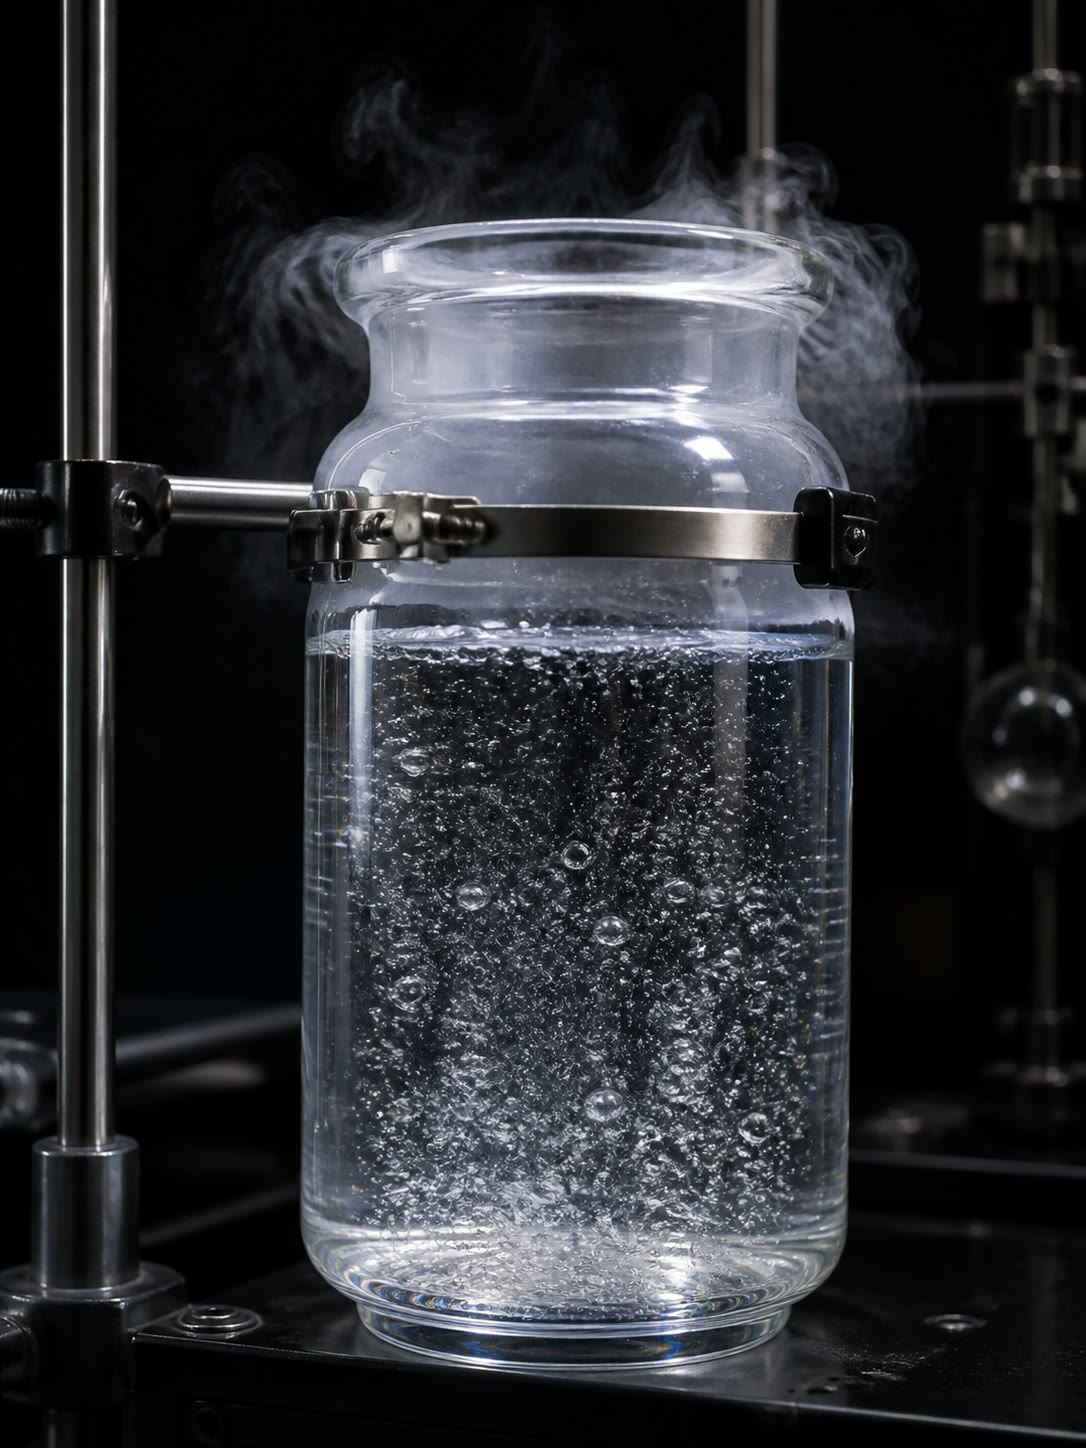
\includegraphics[width=0.45\linewidth]{images/book5/ai/b5-14-liquid-helium-dewar.jpg}

{\small Vloeibaar helium, dat rustig kookt nabij \qty{4}{K}: een vloeistof van volmaakt identieke bosonen. Enkele graden lager houdt het abrupt op met koken en stroomt het zonder wrijving --- ononderscheidbaarheid, tot hydraulica verheven.}
\end{omfigure}

\section{Opgaven}

\begin{exercise}[$\star$]\label{exo:b3:identical-particles:1}
(a) Toon aan dat $\hat P_{12}$ hermitisch is en $\hat P_{12}^2 = \mathbb 1$: wat zijn zijn mogelijke \omterm{def:b3:quantum-formalism:observable}{eigenwaarden}? (b) Toon aan dat $[\hat P_{12}, \hat H] =
0$ voor \omterm{def:b3:identical-particles:exchange}{identieke deeltjes} en concludeer dat de symmetrieklasse
behouden blijft. (c) Waarom kan een toestand van twee \omterm{def:b3:identical-particles:exchange}{identieke deeltjes}
niet eenvoudigweg $\ket a\otimes\ket b$ ``zijn'' zonder symmetrie? (d)
Deel in: $^1$H, $^2$H (deuterium), $^4$He, $^3$He, een waterstofmolecuul,
een foton.
\end{exercise}

\begin{exercise}[$\star$]\label{exo:b3:identical-particles:2}
(a) Schrijf de genormeerde antisymmetrische toestand op die uit
orthogonale orbitalen $\ket a, \ket b$ is gebouwd. (b) Toon aan dat zij
verdwijnt wanneer $a = b$. (c) Voor drie fermionen in $a, b, c$: schrijf
de volledig antisymmetrische combinatie op (zes termen met afwisselende
tekens --- een $3\times3$-determinant) en ga na dat één verwisseling haar
teken omklapt. (d) Waarom maakt de determinantvorm het beginsel van Pauli
vanzelfsprekend?
\end{exercise}

\begin{exercise}[$\star$]\label{exo:b3:identical-particles:3}
Twee deeltjes delen drie orthogonale toestanden. Tel de
tweedeeltjestoestanden voor (a) onderscheidbare deeltjes; (b) bosonen; (c)
fermionen (zonder spin). (d) Herhaal (c) voor elektronen met spin: hoeveel
toestanden nu?
\end{exercise}

\begin{exercise}[$\star$]\label{exo:b3:identical-particles:4}
(a) Geef de grondconfiguraties van koolstof, stikstof, zuurstof en neon.
(b) Formuleer de regel van Hund en pas haar toe op de drie
$2p$-elektronen van stikstof. (c) Rechtvaardig de regel van Hund in één
zin uit \cref{prop:b3:identical-particles:exchange-force}. (d) Welk
element is dankzij zijn volle schillen de traagste stof die men kent, en
welk enkel ontbrekend elektron maakt fluor het gretigst?
\end{exercise}

\begin{exercise}[$\star\star$]\label{exo:b3:identical-particles:5}
Twee niet-wisselwerkende deeltjes in een doos met niveaus $E_n = n^2E_1$.
(a) De grondenergie voor twee bosonen; voor twee fermionen zonder spin;
voor twee elektronen. (b) Het eerste aangeslagen niveau van elk. (c) De
fermionische grondtoestand kost meer: deze ``fermipromotie'' is een druk
in de dop --- leg in één zin uit hoe zij materie belet in te storten. (d)
Veralgemeen: toon aan dat de grondenergie van $N$ fermionen zonder spin in
de doos als $N^3$ groeit en niet als $N$.
\end{exercise}

\begin{exercise}[$\star\star$]\label{exo:b3:identical-particles:6}
Met orthogonale reële orbitalen $\varphi_a, \varphi_b$ en paartoestanden
$\psi_\pm \propto \varphi_a(1)\varphi_b(2) \pm
\varphi_b(1)\varphi_a(2)$: (a) toon aan dat $\psi_-(\vect r, \vect r) = 0$; (b) leid af dat $\langle(\vect r_1 - \vect r_2)^2\rangle_\pm =
(\text{gemeenschappelijke termen}) \mp 2\,|\bra{a}\hat{\vect r}\ket{b}|^2$
en benoem welke symmetrie de deeltjes verder uit elkaar houdt; (c)
beredeneer voor een afstotende wisselwerking $V(|\vect r_1 - \vect r_2|)$
het teken van $E_+ - E_-$; (d) leg het verband met de volgorde van ortho
en para in helium.
\end{exercise}

\begin{exercise}[$\star\star$]\label{exo:b3:identical-particles:7}
De ladder van helium. (a) Waarom moet de grondtoestand een spinsinglet
zijn? (b) Het triplet $1s2s$ ligt \qty{0.80}{eV} onder de singlet $1s2s$:
druk dit uit als een verwisselingsintegraal en vergelijk de omvang ervan
met magnetische spin-spinenergieën ($\sim\mu_{\text{B}}^2\mu_0/4\pi
a_0^3$; reken die uit). (c) Waarom is de toestand $2\,^3S$ metastabiel
(welke twee selectieregels moeten beide worden gebroken)? (d) Haar gemeten
levensduur is $\approx\qty{8000}{s}$: vergelijk met de \qty{1.6}{ns} van
waterstof $2p$ en verbaas u met mate.
\end{exercise}

\begin{exercise}[$\star\star$]\label{exo:b3:identical-particles:8}
Ortho- en parawaterstof. De twee protonen van H$_2$ zijn fermionen: de
\emph{totale} toestand van kernspin $\times$ rotatie moet onder hun
verwisseling antisymmetrisch zijn; de protonen verwisselen keert ook de
molecuulas om, wat de rotatietoestand met $(-1)^J$ vermenigvuldigt. (a)
Toon aan dat het kerntriplet (ortho) bij oneven $J$ hoort en de singlet
(para) bij even $J$. (b) Welke verhouding ortho:para schrijven de
spinmultipliciteiten bij hoge temperatuur voor? (c) De laagste toestand
van ortho ($J = 1$) ligt $2B \approx \qty{15}{meV}$ boven de $J = 0$ van
para, en de spinomzetting duurt dagen: wat gebeurt er in een tank vers
vloeibaar gemaakte waterstof terwijl de orthofractie langzaam omzet, en
waarom moeten vloeibaarmakingsinstallaties de omzetting \emph{vóór} de
opslag katalyseren? (d) Welk alledaags programma met cryogene brandstof
(raketten!) stuit precies op dit probleem?
\end{exercise}

\begin{exercise}[$\star\star$]\label{exo:b3:identical-particles:9}
Bosonische stormloop. Een modus bevat $n$ fotonen; de matrixelementen om
er één toe te voegen schalen als $\sqrt{n+1}$. (a) Toon aan dat de
emissietempo's in de modus als $n + 1$ schalen en de absorptie als $n$.
(b) Vergelijk in een holte waarin één modus $10^{10}$ fotonen bevat en
haar buren geen, de emissietempo's van een aangeslagen atoom in elk
ervan. (c) Leg in twee zinnen uit hoe dit laserlicht in één enkele modus
laat \emph{groeien}. (d) Waar dook de $\sqrt{n+1}$ al op in
\cref{prop:b3:harmonic-oscillator:coherent-motion}?
\end{exercise}

\begin{exercise}[$\star\star\star$]\label{exo:b3:identical-particles:10}
De paradox van Gibbs, opgelost door identiteit. Twee gelijke volumes $V$
ideaal gas met elk $N$ moleculen en dezelfde temperatuur worden verbonden.
(a) Zijn de gassen \emph{verschillend} (zeg argon en neon), dan stijgt de
entropie met $2Nk_{\text{B}}\ln2$ --- haal op waarom (elk gas verdubbelt
zijn volume). (b) Zijn zij \emph{hetzelfde} gas, dan verandert het openen
van de kraan macroscopisch niets: welke ongerijmdheid zou volgen als de
mengentropie toch zou verschijnen (denk aan dichtdoen en weer opendoen)?
(c) Toon aan dat de moleculen als onderscheidbaar behandelen die valse
entropie \emph{wel} voortbrengt, en dat de toestandstelling door $N!$
delen --- alleen geoorloofd omdat de moleculen identiek zijn --- haar
opheft. (d) Moraal, in één zin: de klassieke statistische fysica leent
stilzwijgend een kwantumfeit; de volgende hoofdstukken zullen het luidop
lenen.
\end{exercise}

\begin{exercise}[$\star\star\star$]\label{exo:b3:identical-particles:11}
Pauli houdt de doden overeind. Een witte dwerg propt ongeveer
$\qty{e9}{kg/m^3}$ samen, dat wil zeggen een elektrondichtheid
$n_{\text{e}} \approx
\qty{3e35}{m^{-3}}$ (één elektron per twee
nucleonmassa's). (a) Bereken de fermi-energie met
\cref{exo:b3:schrodinger-three-dimensions:8}
--- en merk op dat de niet-relativistische formule kraakt. (b) Vergelijk
$E_{\text{F}}$ met $k_{\text{B}}T$ bij $T = \qty{e7}{K}$: in welke zin is
deze witgloeiende ster \emph{koud}? (c) Leg in twee zinnen uit hoe de
uitsluiting, en niet de warmte, de druk levert die de zwaartekracht in
evenwicht houdt. (d) Wat moet er gebeuren wanneer er massa bij komt en
$E_{\text{F}}$ relativistisch wordt --- welke beroemde grens kondigt zich
daarmee aan (\cref{ch:b3:astrophysics})?
\end{exercise}

\begin{exercise}[$\star\star\star$]\label{exo:b3:identical-particles:12}
Van verwisseling naar magneten. Modelleer twee naburige elektronen in een
vaste stof met \cref{prop:b3:identical-particles:exchange-force}: hun
energie is $E_{\text{singlet}}$ of $E_{\text{triplet}} =
E_{\text{singlet}} - 2J$ met verwisselingsconstante $J$. (a) Toon aan dat
dit wordt weergegeven door de effectieve spinhamiltoniaan $\hat H =
-2J\,\hat{\vect S}_1\cdot\hat{\vect S}_2/\hbar^2$ (gebruik
$\hat{\vect S}_1\cdot\hat{\vect S}_2 = \tfrac12[\hat S^2 - \hat
S_1^2 - \hat S_2^2]$). (b) Voor $J > 0$ lijnen naburige spins uit: welk
macroscopisch verschijnsel brengt een rooster van zulke paren voort? (c)
Schat de ordeningstemperatuur $k_{\text{B}}T_{\text{C}}
\sim J$ voor $J \approx \qty{0.1}{eV}$ en vergelijk met de \qty{1043}{K} van ijzer. (d)
Waarom kon geen enkele \emph{magnetische} dipool-dipoolwisselwerking (denk
aan haar omvang uit \cref{exo:b3:identical-particles:7}b) een magneet van
duizend kelvin verklaren --- en wat wel, in één zin?
\end{exercise}

\section{Vraagstuk: De logica van het periodiek systeem}

\begin{problem}[{Weekendvraagstuk --- drie kwantumregels bouwen de hele
scheikunde}]\label{pb:b3:identical-particles:1}
Geef een natuurkundige de waterstoforbitalen $(n, l, m)$, de spin van het
elektron en het beginsel van Pauli, en het \omterm{prop:b3:identical-particles:periodic}{periodiek systeem} volgt ---
perioden, families, afmetingen, de zigzag van ionisatie-energieën, zelfs
de kleur van goud. Dit vraagstuk bouwt het op. Gegevens: waterstofachtige
niveaus $-13.6\,Z_{\text{eff}}^2/n^2$ eV; gemeten eerste
ionisatie-energieën (eV): H $13.6$, He $24.6$, Li $5.4$, Be $9.3$, B
$8.3$, C $11.3$, N $14.5$, O $13.6$, F $17.4$, Ne $21.6$, Na $5.1$.

\medskip\noindent\textbf{Deel I --- De drie regels.}
\begin{enumerate}
  \item Noem de drie ingrediënten: de orbitalencatalogus $(n, l, m)$ met
        haar ontaardingen, de verdubbeling door de spin, en het
        uitsluitingsbeginsel. Hoeveel elektronen passen er in $n = 1$,
        $2$ en $3$?
  \item Waarom verschilt de \emph{energievolgorde} van de subschillen in
        een atoom met veel elektronen van de volgorde op zuivere $n$ van
        waterstof (denk aan doordringing en afscherming,
        \cref{exo:b3:hydrogen-atom:8})?
  \item Schrijf de vulvolgorde tot en met $4s$ en $3d$ op, en geef de
        configuraties van Na ($Z = 11$), Cl ($17$), K ($19$) en Fe
        ($26$).
  \item Rijlengten: verklaar de waargenomen $2, 8, 8, 18$ van de eerste
        vier perioden van de tabel uit de vulvolgorde (waarom is de derde
        rij 8 en niet 18?).
  \item Welk enkel kenmerk maakt de edelgassen scheikundig stil?
  \item Definieer de effectieve lading $Z_{\text{eff}}$ die een
        valentie-elektron ziet, en leg uit waarom zij voor het
        buitenelektron van natrium ruwweg $1$ is, terwijl de elektronen
        van helium elk bijna de volle $Z = 2$ min een fractie van
        elkaars afscherming zien.
\end{enumerate}

\medskip\noindent\textbf{Deel II --- De tweede rij lezen.}
\begin{enumerate}[resume]
  \item Uit de gegevens klimt de ionisatie-energie van Li naar Ne, maar
        zakt zij bij B en bij O: wijs beide dalen aan.
  \item Verklaar het dal bij boor (welke subschil gaat bij B open, en
        waarom is $2p$ duurder vast te houden dan $2s$?).
  \item Verklaar het dal bij zuurstof (wat moeten twee van de
        $2p$-elektronen van zuurstof voor het eerst doen, en het comfort
        van welke regel gaat verloren?).
  \item Schat de ionisatie-energie van helium naïef als $13.6 \times Z^2 = \qty{54.4}{eV}$: waarom is de gemeten \qty{24.6}{eV} zoveel
        kleiner, en welk getal $Z_{\text{eff}} \approx 1.34$ vertelt de
        aanpassing u?
  \item De \qty{5.4}{eV} van lithium tegen de \qty{13.6}{eV} van
        waterstof: welk tweetal effecten (afscherming; hogere $n$) spant
        samen?
  \item Waarom \emph{krimpt} de atomaire afmeting over een rij (Li $\to$
        Ne), hoewel er elektronen bij komen?
\end{enumerate}

\medskip\noindent\textbf{Deel III --- Families en bindingen.}
\begin{enumerate}[resume]
  \item Alkalimetalen: één $s$-elektron boven een edelgasromp --- leid
        hun familietrekken (lage ionisatie, ionen $+1$, heftige
        waterchemie) uit de configuratie af.
  \item Halogenen: één gat in een $p$-schil --- leid de hunne af
        (elektronenaffiniteit, ionen $-1$, tweeatomige moleculen).
  \item De vier van koolstof: waarom is een atoom $2s^22p^2$ in de
        praktijk vierwaardig (welke bijna-ontaarding laat het promoveren
        en hybridiseren --- denk aan de starkhybriden van
        \cref{ex:b3:perturbation-theory:stark})?
  \item Gebruik \cref{ex:b3:identical-particles:bond}: waarom vormen twee
        atomen met gesloten schillen (twee heliums) \emph{geen} covalente
        binding?
  \item Overgangsmetalen: de bijna-ontaarding van $4s$ en $3d$ levert
        tien kolommen met vergelijkbare scheikunde op: waarom verandert
        het vullen van een \emph{inwendige} $d$-schil de scheikunde zo
        weinig?
  \item Voorspel uit de configuraties alleen welke van K, Ca en Sc als
        eerste ongepaarde $d$-elektronen vertoont die klaar zijn voor
        magnetisme.
\end{enumerate}

\medskip\noindent\textbf{Deel IV --- Voorbij de vuistregels.}
\begin{enumerate}[resume]
  \item De regel van Hund kent stikstof drie evenwijdige $2p$-spins toe:
        welke meetbare eigenschap van het atoom (zijn magnetische moment)
        legt dat vast, en welk mechanisme uit hoofdstuk 14 betaalt de
        uitlijning?
  \item Het bestaan van de tabel vergt strikte identiteit van de
        elektronen: wat zouden ``licht onderscheidbare'' elektronen met
        het beginsel van Pauli en met het sluiten van de schillen doen?
  \item In zware atomen bewegen de binnenelektronen met $Z\alpha c$:
        schat voor goud ($Z = 79$) de waarde $v/c$ van het paar $1s$ en
        zeg kwalitatief wat de relativiteitstheorie met de energie van de
        orbitaal $6s$ doet --- de aanvaarde verklaring van de kleur van
        goud en de vloeibaarheid van kwik.
  \item De subschil $4s$ vult vóór $3d$ en ioniseert bij
        overgangsmetalen toch het \emph{eerst}, en chroom en koper lenen
        een $s$-elektron om $3d^5$ en $3d^{10}$ te halen: wat zeggen deze
        afwijkingen over hoe dicht de energieën van de twee subschillen
        bij elkaar liggen?
  \item Twee isotopen van een element zijn scheikundig vrijwel identiek:
        waarom bekommert de scheikunde zich volgens de drie regels alleen
        om $Z$ en nauwelijks om de massa van de kern?
  \item Periode 7 eindigt nabij $Z \approx 118$ en de scheikunde van de
        superzware elementen wijkt af van de naïeve kolomlogica van de
        tabel: noem de twee concurrerende schalen (de schilstructuur
        tegenover de relativistische en coulombse effecten bij grote
        $Z$).
  \item Vat het genoemde resultaat samen: één catalogus van orbitalen,
        één verdubbeling door de spin, één minteken --- en de uitkomst is
        de periodieke wet: rijen $2, 8, 8, 18$, de dalen bij B en O, de
        families van de reactieve en de edele elementen, alle gemeten in
        de ionisatieladder van \qty{5.1}{eV} (Na) tot \qty{24.6}{eV}
        (He).
\end{enumerate}
\end{problem}
